% include all necessary latex libraries
\documentclass[aspectratio=169,presentation]{beamer}
\usetheme{Boadilla}
\useinnertheme{default}

% -- locale-setup --------------------------------------------------------------

\usepackage[utf8]{inputenc}
\usepackage[T1]{fontenc}
\usepackage[ngerman]{babel}
\usepackage{lmodern}
\usepackage[locale=DE, mode=math, list-final-separator={ oder },
            range-phrase={ bis }, scientific-notation=false, 
            group-digits=integer] {siunitx}

% -- package-includes ----------------------------------------------------------

\usepackage{tikz}
\usepackage{xcolor}
\usetikzlibrary{positioning,automata,matrix,arrows.meta,fit}
\usepackage{graphicx} % including images
\usepackage[font=small,labelfont=bf]{caption} % captions of tables and figures

% -- listing setup -------------------------------------------------------------

\usepackage{listings}
\definecolor{pblue}{rgb}{0.13,0.13,1}
\definecolor{pgreen}{rgb}{0,0.5,0}
\definecolor{pred}{rgb}{0.9,0,0}
\definecolor{pgrey}{rgb}{0.46,0.45,0.48}
\definecolor{javared}{rgb}{0.6,0,0} % for strings
\definecolor{javagreen}{rgb}{0.25,0.5,0.35} % comments
\definecolor{javapurple}{rgb}{0.5,0,0.35} % keywords
\definecolor{javadocblue}{rgb}{0.25,0.35,0.75} % javadoc

\lstset{language=vhdl,
	basicstyle=\ttfamily,
	keywordstyle=\color{javapurple}\bfseries,
	stringstyle=\color{javared},
	commentstyle=\color{javagreen},
	morecomment=[s][\color{javadocblue}]{/**}{*/},
	tabsize=2,
	showspaces=false,
	showstringspaces=false
}

% -- custom commands -----------------------------------------------------------

% just prints given text in large text and on empty frame.
\newcommand{\sectionframe} [1] {
	\begin{frame}
		\vfill
		\Huge
		\centering
		\usebeamercolor[fg]{title}
		#1
		\vfill
		\par
	\end{frame}
}

% wrapper-command to make pretty title takes
% 1=short-title 2=long-title 3=terminnumber 4=date
\newcommand{\maketitlepage} [5] {
  \title[#1]{#2}
  \subtitle{Termin #3}
  \date{#4}
  \author[Jakob Otto]{Jakob Otto}
  \institute{HAW Hamburg}
  \subject{#1}
  \pgfdeclareimage[height=0.5cm, width=1.3cm]{university-logo}{#5}
  \logo{\href{https://www.haw-hamburg.de}{\pgfuseimage{university-logo}}}
  \begin{frame} {}
    \titlepage
  \end{frame}
}

% draws a link symbol
\newcommand{\externalLink} {
  \tikz[x=1.2ex, y=1.2ex, baseline=-0.05ex]{
    \begin{scope}[x=1ex, y=1ex]
      \clip (-0.1,-0.1) 
        --++ (-0, 1.2) 
        --++ (0.6, 0) 
        --++ (0, -0.6) 
        --++ (0.6, 0) 
        --++ (0, -1);
      \path[draw, 
        line width = 0.5, 
        rounded corners=0.5] 
      (0,0) rectangle (1,1);
    \end{scope}
      \path[draw, line width = 0.5] (0.5, 0.5) 
        -- (1, 1);
    \path[draw, line width = 0.5] (0.6, 1) 
      -- (1, 1) -- (1, 0.6);
  }
}

% Adds a circled number -> Looks better than the default
\newcommand{\circled} [1] {
  \tikz[baseline=(char.base)]{
    \node[shape=circle,draw,inner sep=2pt, text centered, text width = .2cm] (char) {#1};
  }
}

% -- extra includes go here ----------------------------------------------------
\usepackage{tikz}
\usepackage[customcolors]{hf-tikz}
\usetikzlibrary{shapes,arrows, positioning, fit, backgrounds}

\newcommand{\connectlr} [3] {
  \path (#1.east) -- (#1.north east) coordinate[pos=0.5] (tmp11);
  \path (#2.west) -- (#2.north west) coordinate[pos=0.5] (tmp21);
  \draw[-latex] (tmp21) -- (tmp11);
  \path (#1.east) -- (#1.south east) coordinate[pos=0.5] (tmp12);
  \path (#2.west) -- (#2.south west) coordinate[pos=0.5] (tmp22);
  \draw[-latex] (tmp12) -- (tmp22);
  \path (#1) -- (#2) node [midway] {\circled{#3}};
}

\newcommand{\connecttb} [3] {  
  \path (#1.south) -- (#1.south west) coordinate[pos=0.5] (tmp11);
  \path (#2.north) -- (#2.north west) coordinate[pos=0.5] (tmp21);
  \draw[-latex] (tmp21) -- (tmp11);
  \path (#1.south) -- (#1.south east) coordinate[pos=0.5] (tmp12);
  \path (#2.north) -- (#2.north east) coordinate[pos=0.5] (tmp22);
  \draw[-latex] (tmp12) -- (tmp22);
  \path (#1) -- (#2) node [midway] {\circled{#3}};
}

% put color to \boxed math command
\newcommand*{\boxcolor}{orange}
\makeatletter
\renewcommand{\boxed}[2]{\textcolor{#1}{%
\tikz[baseline={([yshift=-1ex]current bounding box.center)}] \node [rectangle, minimum width=1ex,rounded corners,draw] {\normalcolor\m@th$\displaystyle#2$};}}
 \makeatother

%-------------------------------------------------------------------------------
%	Variablen
%-------------------------------------------------------------------------------

\newcommand{\terminnumber}{2}
\newcommand{\hawlogo}{../presentation-template/figs/logo-haw-2017}
\newcommand{\kratzen}{../presentation-template/figs/kratzen}
\newcommand{\aufgabenzettellink}{https://users.informatik.haw-hamburg.de/~schafers/LOCAL/S19W_CE/Aufgabenzettel_Nr2_v10.pdf}

%-------------------------------------------------------------------------------
%	Dokument
%-------------------------------------------------------------------------------

\begin{document}
  \maketitlepage {CE Tutorium} {Tutorium zu\\Computer-Engineering\\im SS19} 
                 {\terminnumber} {\today} {\hawlogo}

  %-----------------------------------------------------------------------------
  %	Ablauf
  %-----------------------------------------------------------------------------

  \section{Ablauf}
  \begin{frame}{Ablauf}
    \begin{columns}
      \column{0.4\textwidth}
        \begin{itemize}
          \item Ausblick
          \item Praktikumsaufgabe
          \begin{itemize}
            \item Trial-subtraction-Verfahren
            \item Tipps
            \item Testen
          \end{itemize}
        \end{itemize}
      \column{0.6\textwidth}
        \begin{center}
          
\includegraphics[width=.6\textwidth] {\kratzen}
        \end{center}
    \end{columns}
  \end{frame}

  %-----------------------------------------------------------------------------
  %	Ausblick
  %-----------------------------------------------------------------------------

  \section{Ausblick}
  \begin{frame} {Ausblick (I)}
    \begin{block} {Ablauf}
      \begin{enumerate}
        \item Trial-Subtraction Algorithmus
        \begin{itemize}
          \item effizientes Wurzelziehen aus Samples
        \end{itemize}
        \item DAC spielereien
        \begin{itemize}
          \item Ausgabe von Sound lernen
        \end{itemize}
        \item Flash-speicher lesen/schreiben
        \begin{itemize}
          \item Samples lesen lernen
        \end{itemize}
        \item Alles zusammensetzen
        \begin{itemize}
          \item Kommunikation zwischen FPGA/STM-32
          \item Ausgabe übr PWM
          \item Musik abspielen
        \end{itemize}
      \end{enumerate}
    \end{block}
  \end{frame}

  \begin{frame} {Ausblick (II)}
    % Define a few styles and constants
    \tikzstyle{block} = [text width=6em, text centered, minimum height=6em, 
                         rounded corners, draw]
    \tikzstyle{stm32} = [fill=red!20, block]
    \tikzstyle{fpga}=[fill=blue!20, block]
    \tikzstyle{flash}=[fill=green!20, block]
    \tikzstyle{output}=[fill=yellow!20, block]
    \begin{center}
      \begin{tikzpicture} [node distance=5cm]
        \node (stm32) [stm32] {STM-32};
        \node (fpga) [fpga, left of = stm32] {FPGA};
        \node (flash) [flash, below of = stm32] {flash-memory};
        \node (output) [output, right of = stm32] {PWM/\\DAC};
        \node (legend) [below of=output,fill=white, draw, text width=5cm] {
          \circled{1} Samples beschaffen\\
          \circled{2} Wurzel ziehen\\
          \circled{3} ausgeben
        };
        % -- connect fpga and stm32 --------------------------------------------
        \connectlr {fpga} {stm32} {2}
        \connectlr {stm32} {output} {3}
        \connecttb {stm32} {flash} {1}
      \end{tikzpicture}
    \end{center}
  \end{frame}

  \begin{frame} {Ausblick (III)}
    \tikzstyle{block} = [text width=6em, text centered, minimum height=6em, 
                         rounded corners, draw]
    \tikzstyle{stm32} = [fill=red!20, block]
    \tikzstyle{fpga}=[fill=blue!20, block]
    \tikzstyle{flash}=[fill=green!20, block]
    \tikzstyle{output}=[fill=yellow!20, block]
    \tikzstyle{surround} = [fill=white,thick,draw=red,rounded corners=2mm]
    \begin{center}
      \begin{tikzpicture} [node distance=5cm]
        \node (stm32) [stm32] {STM-32};
        \node (fpga) [fpga, left of = stm32] {FPGA};
        \node (flash) [flash, below of = stm32] {flash-memory};
        \node (output) [output, right of = stm32] {PWM/\\DAC};
        \node (legend) [below of=output,fill=white, draw, text width=5cm] {
          \circled{1} Samples beschaffen\\
          \circled{2} Wurzel ziehen\\
          \circled{3} ausgeben
        };
        \begin{pgfonlayer}{background} 
          \node[surround] (background) [fit = (fpga)] {};
        \end{pgfonlayer}
        % -- connect fpga and stm32 --------------------------------------------
        \connectlr {fpga} {stm32} {2}
        \connectlr {stm32} {output} {3}
        \connecttb {stm32} {flash} {1}
      \end{tikzpicture}
    \end{center}
  \end{frame}
  
  %-----------------------------------------------------------------------------
  %	Praktkumsaufgabe
  %-----------------------------------------------------------------------------

  \section{Praktikumsaufgabe}
  \sectionframe{\href{\aufgabenzettellink}{Aufgabenzettel\externalLink}}
  
  \section{Aufgabe}
  \begin{frame} {Praktikum (I)}
    \begin{block} {Warum eigentlich?}
      \begin{itemize}
        \item Wurzelziehen ist teuer
        \item Hardware-unterstützung hilfreich
        \item Bei uns durch Trial-Subtraction Algorithmus realisiert
      \end{itemize}
    \end{block}
  \end{frame}

  \begin{frame} {Praktikum (II)}
    \begin{block} {Warum eigentlich?}
      \begin{center}
        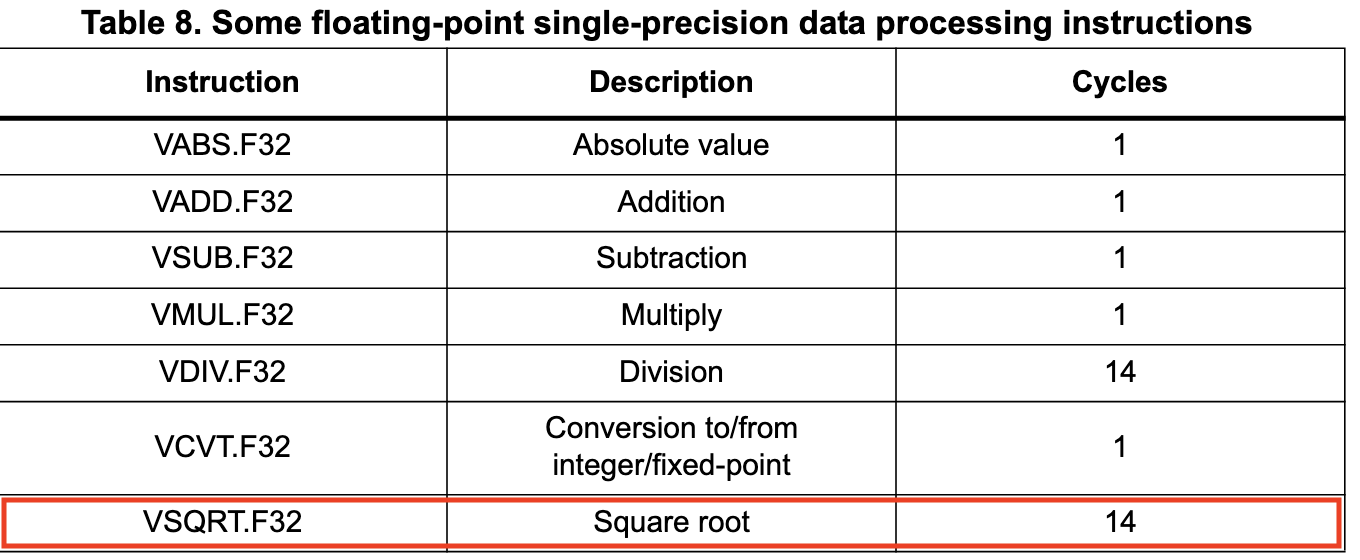
\includegraphics[width=.7\textwidth]{figs/arith_cycles.png}
      \end{center}
    \end{block}
  \end{frame}

  \begin{frame} {Praktikum (III)}
    \begin{block} {Einschränkungen...}
      \begin{itemize}
        \item Wir sind Stückkosten getrieben!
        \item Daher \textbf{\underline{ein}} Addierer und 
              \textbf{\underline{ein}} Subtrahierer erlaubt
        \begin{itemize}
          \item Addierer für Inkrementieren des Zustands
          \item Subtrahierer für Algorithmus
        \end{itemize}    
      \end{itemize}
    \end{block}
    \begin{alertblock} {}
      Denkt an Aufgabe 3 aus DT $\rightarrow$ Addierer richtig einsetzen!
    \end{alertblock}
  \end{frame}

  \begin{frame} [fragile] {Kleine Erinnerung (I)}
    \begin{alertblock} {}
      \textbf{SO NICHT!!}
    \end{alertblock}
    \begin{lstlisting}
add: process (a_s, b_s, c_s, select_s) is 
  variable res_v : <type>;
begin
  if (select_s = '0') then
    res_v := a_s + b_s;
  else
    res_v := b_s + c_s;
  end if;

  res_s <= res_v;
end process;
    \end{lstlisting}
  \end{frame}

  \begin{frame} [fragile] {Kleine Erinnerung (II)}
    \begin{exampleblock} {}
      \textbf{BESSER}
    \end{exampleblock}    
    \begin{lstlisting}
add: process (a_s, b_s, c_s, select_s) is 
  -- variablen opA_v, opB_v, res_v
begin
  if (select_s = '0') then
    opA_v := a_v;
    opB_v := b_v;
  else
    opA_v := b_v;
    opB_v := c_v;
  end if;

  res_v := opA_v + opB_v
  res_s <= res_v;
end process;
    \end{lstlisting}
  \end{frame}

  %-----------------------------------------------------------------------------
  %	Trial-Subtraction Algorithmus
  %-----------------------------------------------------------------------------

  \section{Trial-Subtraction Algorithmus}
  \begin{frame} {Trial-Subtraction Algorithmus (I)}
    \begin{block} {Ablauf}
      \begin{enumerate}
        \item n = 1
        \item $r'$ und $s'$ berechnen
        \item wenn:
        \begin{enumerate}
          \item r' >= 0 $\rightarrow$ s = s'
          \item r' ~< ~0 $\rightarrow$ s = s
        \end{enumerate}
        \item sobald:
        \begin{enumerate}
          \item r' = 0 $\rightarrow$ \textbf{ende}
          \item sonst $\rightarrow$ $n = n + 1$ und gehe zu 2
        \end{enumerate} 
      \end{enumerate}
    \end{block}
  \end{frame}

  \begin{frame} {Trial-Subtraction Algorithmus (II)}
    \begin{block} {Variablen}
      \begin{itemize}
        \item $s$ $\rightarrow$ Approximation der Wurzel
        \item $s'$ $\rightarrow$ die neue Approximation
        \item $r$ $\rightarrow$ der mögliche Rest
        \item $r'$ $\rightarrow$ ein möglicher neuer Rest
        \item $n$ $\rightarrow$ Der Zustand/die Phase
        \item $d$ $\rightarrow$ Differenz $\rightarrow 2^n$
      \end{itemize}
    \end{block}
  \end{frame}

  \begin{frame} {Trial-Subtraction Algorithmus (II)}
    \begin{block} {Funktionen}
      \begin{align*}
        r' &= r - 2^n (2s + 2^n) \\
        s' &= s + 2^n
      \end{align*}
    \end{block}
  \end{frame}

  \begin{frame} {Trial-Subtraction Algorithmus (III)}
    \begin{block} {Ursprüngliche Funktion}
      \begin{equation*}
        r' = r - \boxed{red}{2^n\cdot}\boxed{blue}{(2s + 2^n)}
      \end{equation*}
    \end{block}

    \begin{exampleblock} {}
      Multiplikation mit 2 lässt sich durch shift darstellen \\
      Addition in diesem Fall durch '|'
    \end{exampleblock}
    \begin{block} {Vereinfacht}
      \hfsetfillcolor{green!10}
      \hfsetbordercolor{green!50!black}
      \begin{equation*}
        r' = r - (\boxed{blue}{((s << 1)~|~(1 << n))} \boxed{red}{<< n})
      \end{equation*}
    \end{block}
  \end{frame}

  \begin{frame} {Trial-Subtraction Algorithmus (IV)}
    \begin{block} {Ursprüngliche Funktion}
      \begin{equation*}
        s' = s + 2^n
      \end{equation*}
    \end{block}
    \begin{exampleblock} {}
      Multiplikation mit 2 lässt sich durch shift darstellen \\
      Addition in diesem Fall durch '|'
    \end{exampleblock}
    \begin{block} {Vereinfacht}
      \begin{equation*}
        s' = s~|~(1 << n)
      \end{equation*}
    \end{block}
  \end{frame}

  \begin{frame} {Trial-Subtraction Algorithmus (V)}
    \begin{block} {Bei uns etwas anders...}
      \begin{itemize}
        \item Wir ziehen wurzel aus $Q_{0.15}$ Format
        \begin{itemize}
          \item Zahlenbereich von $-1 \dots \sim{}1$
          \item In der Rechnung nur $0 \dots 1$
        \end{itemize}
        \item Logik daher etwas anders
        \begin{itemize}
          \item Statt $2^n \rightarrow 2^{-n}$
          \item $0.5, 0.25, 0.125, \dots$
        \end{itemize}
      \end{itemize}
    \end{block}
  \end{frame}

  \begin{frame} {Trial-Subtraction Algorithmus (VI)}
    \begin{block} {Eigentlich}
      \begin{align*}
        r' &= r - (((s << 1)~|~(1 << n)) >> n) \\
        s' &= s~|~(1 << n)
      \end{align*}
    \end{block}
    \begin{exampleblock} {Wird zu}
      \begin{align*}
        r' &= r - (((s << 1)~|~(1000000000000000 >> n)) >> n) \\
        s' &= s~|~(1000000000000000 >> n)
      \end{align*}
    \end{exampleblock}
  \end{frame}

  \begin{frame} {Trial-Subtraction Algorithmus (VII)}
    \begin{block} {Eigentlich}
      \begin{align*}
        r' &= r - (((s << 1)~|~(1000000000000000 >> n)) >> n) \\
        s' &= s~|~(1000000000000000 >> n)    
      \end{align*}
    \end{block}
    \begin{exampleblock} {lässt sich noch verbessern}
      \begin{align*}
        d  &= (1000000000000000 >> n) \\
        r' &= r - (((s << 1)~|~d) >> n) \\
        s' &= s~|~d    
      \end{align*}
    \end{exampleblock}    
  \end{frame}

  \begin{frame} [fragile] {Trial-Subtraction Algorithmus (VIII)}
    \begin{exampleblock} {}
      Als Codebeispiel...
    \end{exampleblock}
    \begin{lstlisting}
delta_v := to_stdlogicvector("1000000000000000" srl n_v);
operandB_v := to_stdlogicvector(to_bitvector(
        (s_v(msbPos-1 downto 0) & '0') or (delta_v)) srl n_v);
operandA_v := r_v;
result_v := opA_v - opB_v;
-- weiter interpretieren
    \end{lstlisting}
  \end{frame}

  %-----------------------------------------------------------------------------
  %	Tipps
  %-----------------------------------------------------------------------------

  \section{Tipps}
  \begin{frame} {Tipps (I)}
    \begin{block} {Kein Modularisieren}
      \begin{itemize}
        \item Versucht \textbf{NICHT} den Code modular zu gestalten
        \begin{itemize}
          \item Ein Prozess, der die gesamte Logik enthält
        \end{itemize} 
        \item Modularisieren ist gut, allerdings 40 Zustände dadurch schwer
      \end{itemize}
    \end{block}
  \end{frame}

  \begin{frame} {Tipps (II)}
    \begin{alertblock} {Wichtig!}
      \begin{itemize}
        \item Bevor ihr eine Berechnung startet (Phase 0):
        \begin{itemize}
          \item Eingabe auf VZ prüfen und ggf. positiv machen. $\rightarrow 
                (0-Wert)$ \textbf{VZ merken!}
        \end{itemize} 
        \item Nach der Berechnung Ergebnis wieder Negativ machen $\rightarrow 
              (0-Ergebnis)$
      \end{itemize}
    \end{alertblock}    
  \end{frame}

  \begin{frame} {Tipps (III)}
    \begin{block} {Eingaben}
      \begin{itemize}
        \item Was tun mit Eingaben wie:
        \begin{itemize}
          \item -1 $\rightarrow$ "1000000000000000"
          \item ~0 $\rightarrow$ "0000000000000000"
        \end{itemize}
        \pause
        \item[] Einfach durchreichen
        \item Was ist mit der 1??? 
      \end{itemize}	
    \end{block}
  \end{frame}

  %-----------------------------------------------------------------------------
  %	Testen
  %-----------------------------------------------------------------------------

  \section{Testen}
  \begin{frame} [fragile] {Testen}
    \begin{lstlisting}
for i in -32768 to 32767 loop
  x_s <= std_logic_vector(to_signed(i, x_s'length));
  req_s <= '1'; 

  -- warten, dass Berechnung gestartet wurde
  wait for fullClockCycle;
  req_s <= '0';

  -- warten auf Ende der Berechnung
  wait for 18 * fullClockCycle;
end loop;
    \end{lstlisting}
  \end{frame}

  \section{Ende}
  \begin{frame} {Ende}
    \begin{block} {Nächstes mal}
      \begin{itemize}
        \item Aufgabe 3?
        \item Andere Wünsche?
      \end{itemize}
    \end{block}
    \begin{exampleblock}{Abschließendes}
      Fragen, Anmerkungen und Verbesserungen ausdrücklich erwünscht.\\
      Ich bin auf euer Feedback angewiesen.
    \end{exampleblock}
  \end{frame}

\end{document}